
\documentclass[aps,twocolumn,secnumarabic,nobalancelastpage,amsmath,amssymb,
nofootinbib]{revtex4}

% nofootinbib is another document class option that allows you to put
% footnotes on the page where they occur rather than at the end of the
% paper.  This makes for easier reading!

% secnumarabic is a particularly nice way of identifying sections by
% number to aid electronic review and commentary.

% amsmath and amssymb are necessary for the subequations environment
% among others

\usepackage{chapterbib}
\usepackage{color}
\usepackage{graphics}      % standard graphics specifications
\usepackage{graphicx}      % alternative graphics specifications
\usepackage{longtable}     % helps with long table options
%\usepackage{url}          % for on-line citations (conflicts with hyperref)
\usepackage{bm}            % special 'bold-math' package
\usepackage[colorlinks=true]{hyperref}


\begin{document}
\title{Radioactive Decay}
\author         {Adnan Basar (Partner: Kadir Simsek)}
\email          {adnanbasarr@icloud.com}
\affiliation    {2010205108}
\date{\today}





\begin{abstract}
A radioactive species is often characterized by its half‐life ${t}_{\frac{1}{2}}$, which is defined as the time it takes for one‐half of the nuclei to decay. In this experiment, we are going to calculate half-life of Radon gas.
\end{abstract}

\maketitle

%%%%%%%%%%%%%%%%%%%%%%%%%%%%%%%%%%%%%%%%%%%%%%%%%%%%%%%%%%%%%%%%%%
\section{Introduction}
The rate at which a particular radioactive material disintegrates in a given time interval is called the
decay constant $\lambda$. The decay constant is characteristic of the particular nuclear species and is
independent of all external physical and chemical conditions. Radioactive decay is a statistical process as
one cannot predict when any individual nucleus will decay. The most that one can know is that the
probability that a nucleus will decay in a small time interval $dt$ is $\lambda{dt}$.\\

When a large number of nuclei of a single species are studied, statistics can be used to make definite
predictions aboutthe average number of decaysthat occurin a small time interval. Let $N(t)$ be the total
number of undecayed nuclei at time $t$. If one studied many identically prepared samples, the average
number of decays that occur every second $\frac{dN}{dt}$ is given by

\begin{center}

$\frac{dN}{dt}=-\lambda{N(t)}$

\end{center}

This can be integrated to give the number of undecayed nuclei at time $t$

\begin{center}

$N(t)={N}_{0}{e}^{-\lambda{t}}$


\end{center}

Here ${N}_{0}$ is the number of nuclei present at $t=0$.\\

Using the equation for $N(t)$ we see that ${t}_{\frac{1}{2}}$   satisfies 

\begin{center}

$\frac{N}{{N}_{0}}=\frac{1}{2}={e}^{-\lambda{{t}{\frac{1}{2}}}}$ $\Longrightarrow$ ${t}_{\frac{1}{2}}=\frac{ln2}{\lambda}$

\end{center}

\section{Experimental Setup}

\begin{itemize}
\item Wulf's Electroscope 
\item Thorium Salt
\item Ionization Chamber
\item HV Power Supply (0-5 kV)
\item Stopwatch
\end{itemize}

\section{Data and Analysis}
In data analysis part, we have $S_{i}$ and $T_{i}$ values by using discharge time $t_{i}$ where:

\begin{center}
${S}_{i}= {t}_{i+1}- {t}_{i} $
\end{center}



\begin{center}
${T}_{i}=\frac{{t}_{i+1}+{t}_{i}}{2}$
\end{center}.

\begin{center}
\begin{table}[htbp]
\begin{tabular}{|l|c|c|r|}
\hline
{\small Squeeze Number} & { \small ${S}_{i}$} & {\small  ${T}_{i} $ } \\
\hline
6& 17.0 sec & 8.5 sec  \\
6& 34.0 sec & 34.0 sec  \\
6& 60.0 sec & 81.0 sec  \\
8& 25.0 sec & 12.5 sec  \\
8& 47.0 sec & 53.5 sec  \\
10& 21.0 sec & 10.5 sec  \\
10& 40.0 sec & 42.0 sec  \\
10& 87.0 sec & 104.5 sec  \\
11& 22.0 sec & 11.0 sec  \\
11& 44.0 sec & 44.0 sec  \\
11& 84.0 sec & 98.0 sec  \\


\hline
\end{tabular}
\caption{\label{tab:linfitresults} Values for Voltage 2500 V }
\end{table}
\end{center}

\begin{center}
\begin{table}[htbp]
\begin{tabular}{|l|c|c|r|}
\hline
{\small Squeeze Number} & { \small ${S}_{i}$} & {\small  ${T}_{i} $ } \\
\hline
6& 10.0 sec & 5.0 sec  \\
6& 37.0 sec & 18.5 sec  \\
6& 69.0 sec & 81.5 sec  \\
8& 20.0 sec & 10.0 sec  \\
8& 53.0 sec & 46.5 sec  \\
8& 170.0 sec & 158.0 sec  \\
10& 13.0 sec & 6.5 sec  \\
10& 84.0 sec & 55.0 sec  \\
10& 177.0 sec & 185.5 sec  \\
11& 11.0 sec & 5.5 sec  \\
11& 41.0 sec & 31.5 sec  \\
11& 153.0 sec & 128.5 sec  \\



\hline
\end{tabular}
\caption{\label{tab:linfitresults} Values for Voltage 3000 V }
\end{table}
\end{center}



\begin{center}
\begin{table}[htbp]
\begin{tabular}{|l|c|c|r|}
\hline
{\small Squeeze Number} & { \small ${S}_{i}$} & {\small  ${T}_{i} $ } \\
\hline
6& 5.0 sec & 2.5 sec  \\
6& 39.0 sec & 19.5 sec  \\
6& 83.0 sec & 85.5 sec  \\
8& 12.0 sec & 6.0 sec  \\
8& 37.0 sec & 30.5 sec  \\
8& 125.0 sec & 112.5 sec  \\
10& 6.0 sec & 3.0 sec  \\
10& 34.0 sec & 23.0 sec  \\
10& 67.0 sec & 73.5 sec  \\
11& 4.0 sec & 2.0 sec  \\
11& 43.0 sec & 18.5 sec  \\
11& 116.0 sec & 81.0 sec  \\


\hline
\end{tabular}
\caption{\label{tab:linfitresults} Values for Voltage 3500 V }
\end{table}
\end{center}

\begin{center}
\begin{table}[htbp]
\begin{tabular}{|l|c|c|r|}
\hline
{\small Squeeze Number} & { \small ${S}_{i}$} & {\small  ${T}_{i} $ } \\
\hline
6& 31.0 sec & 16.5 sec  \\
6& 61.0 sec & 61.5 sec  \\
8& 19.0 sec & 8.5 sec  \\
8& 44.0 sec & 41.0 sec  \\
8& 106.0 sec & 116.0 sec  \\
10& 24.0 sec & 12.0sec  \\
10& 45.0 sec & 46.5 sec  \\
10& 106.0 sec & 122.0 sec  \\
11& 15.0 sec & 7.5 sec  \\
11& 32.0 sec & 31.0 sec  \\
11& 54.0 sec & 74.0 sec  \\


\hline
\end{tabular}
\caption{\label{tab:linfitresults} Values for Voltage 4000 V }
\end{table}
\end{center}

\begin{center}
\begin{table}[htbp]
\begin{tabular}{|l|c|c|r|}
\hline
{\small Squeeze Number} & { \small ${S}_{i}$} & {\small  ${T}_{i} $ } \\
\hline
6& 10.0 sec & 5.0 sec  \\
6& 37.0 sec & 18.5 sec  \\
6& 117.0 sec & 82.0 sec  \\
8& 15.0 sec & 7.5 sec  \\
8& 37.0 sec & 36.5 sec  \\
8& 97.0 sec & 106.5 sec  \\
10& 8.0 sec & 4.0 sec  \\
10& 32.0 sec & 24.0 sec  \\
10& 52.0 sec & 66.0 sec  \\
10& 192.0 sec & 188.0 sec  \\
11& 12.0 sec & 6.0 sec  \\
11& 34.0 sec & 29.0 sec  \\
11& 67.0 sec & 79.5 sec  \\


\hline
\end{tabular}
\caption{\label{tab:linfitresults} Values for Voltage 4500 V }
\end{table}
\end{center}

And bu using linear fitting  for specific voltage and squeeze number, we will have 20 $\lambda$ and $\sigma_{\lambda}$. Fitting to 

\begin{center}
$lnS=ln{S}_{0}+{\lambda}{T}$
\end{center}

where $y=lnS$ and error propagation for ${\sigma}_{lnS}$

\begin{center}
${ { \sigma  }_{ y } }^{ 2 }={ { \sigma  }_{ lnS } }^{ 2 }={ \left( \frac { d }{ dS } \left( lnS \right)  \right)  }^{ 2 }{ { \sigma  }_{ S } }^{ 2 }=\frac { 2 }{ { s }^{ 2 } } $
\end{center}

where ${\sigma}_{S}=\sqrt{2}$.

\begin{center}
\begin{table}[htbp]
\begin{tabular}{|l|c|c|r|}
\hline
{\small Voltage}&{\small Squeeze Number} & { \small $\lambda$} & {\small  ${\sigma}_{\lambda} $ } \\
\hline
2500 V&6& 0.014 & 0.00082 \\
3000 V&6& 0.011 & 0.00066  \\
3500 V&6& 0.012 & 0.0006  \\
4000 V&6& 0.015 & 0.00114  \\
4500 V&6& 0.019 & 0.0006  \\

2500 V&8& 0.015 & 0.00156 \\
3000 V&8& 0.011 & 0.00023  \\
3500 V&8& 0.012 & 0.00034  \\
4000 V&8& 0.013 & 0.0004  \\
4500 V&8& 0.015 & 0.00051  \\

2500 V&10& 0.014 & 0.0005 \\
3000 V&10& 0.006 & 0.00014  \\
3500 V&10& 0.015 & 0.0009  \\
4000 V&10& 0.012 & 0.00036  \\
4500 V&10& 0.011 & 0.00018  \\

2500 V&11& 0.013 & 0.00053 \\
3000 V&11& 0.016 & 0.00035  \\
3500 V&11& 0.014 & 0.00056  \\
4000 V&11& 0.015 & 0.00099  \\
4500 V&11& 0.016 & 0.00083  \\





\hline
\end{tabular}
\caption{\label{tab:linfitresults} Fitted $\lambda$ values where ${\sigma}_{\lambda}={\sigma}_{{a}_{1}}$ }
\end{table}
\end{center}




After fitting, we have 20 $\lambda$ and 20 $\sigma_{\lambda}$. By using these values, weighed values and errors can be calculated as:

\begin{center}
${ \lambda  }_{ w }=\frac { \sum _{ i=1 }^{ 20 }{ \frac { { \lambda  }_{ i } }{ { { \sigma  }_{ i } }^{ 2 } }  }  }{ \sum _{ i=1 }^{ 20 }{ \frac { 1 }{ { { \sigma  }_{ i } }^{ 2 } }  }  } $
\end{center}

and 

\begin{center}
${ { \sigma  }_{ { \lambda  }_{ w } } }^{ 2 }=\frac { 1 }{ \sum _{ i=1 }^{ 20 }{ \frac { 1 }{ { { \sigma  }_{ i } }^{ 2 } }  }  } $
\end{center}

From weighted values of $\lambda$, we can measure ${t}_{\frac{1}{2}}$:

\begin{center}
${t}_{\frac{1}{2}}$ $\longrightarrow$ ${t}_{\frac{1}{2}}=\frac{ln2}{{\lambda}_{w}}$
\end{center}

and error of ${t}_{\frac{1}{2}}$:

\begin{center}
${ { \sigma  }_{ { t }_{ \frac { 1 }{ 2 }  } } }^{ 2 }={ \left( \frac { d }{ d\lambda  } \left( { t }_{ \frac { 1 }{ 2 }  } \right)  \right)  }^{ 2 }{ { \sigma  }_{ { \lambda  }_{ w } } }^{ 2 }$
\end{center}

\section{Results}

\begin{center}
$\lambda_{w}=0.0104$\\
${\sigma}_{{\lambda}_{w}}=0.0088$\\
${t}_{\frac{1}{2}}=66.12 $ sec\\
${{\sigma}_{{t}_{\frac{1}{2}}}}^{2}=0.24$ sec \\

\end{center}

Error of ${t}_{\frac{1}{2}}$:

\begin{center}
$Error=\frac{|66.12-55.6|}{0.48}=21.47$ $\gg$ $1\sigma$.
\end{center}



\begin{figure}[htbp]
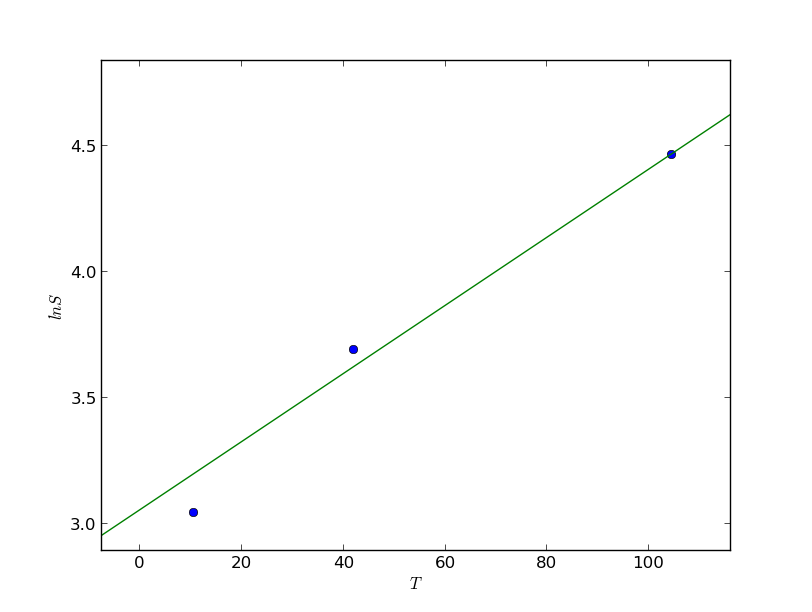
\includegraphics[width=2.5in]{plot1}
\caption{LSF to straight line}
\label{fig:schematic}
\end{figure}

\begin{figure}[htbp]
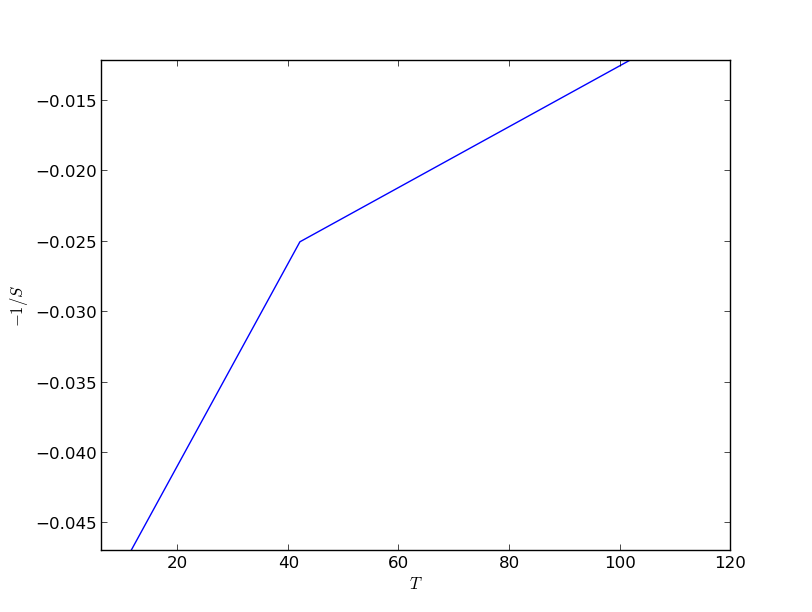
\includegraphics[width=2.5in]{plot2}
\caption{$\frac{-1}{S}$ versus $T$}
\label{fig:schematic}
\end{figure}

\begin{figure}[htbp]
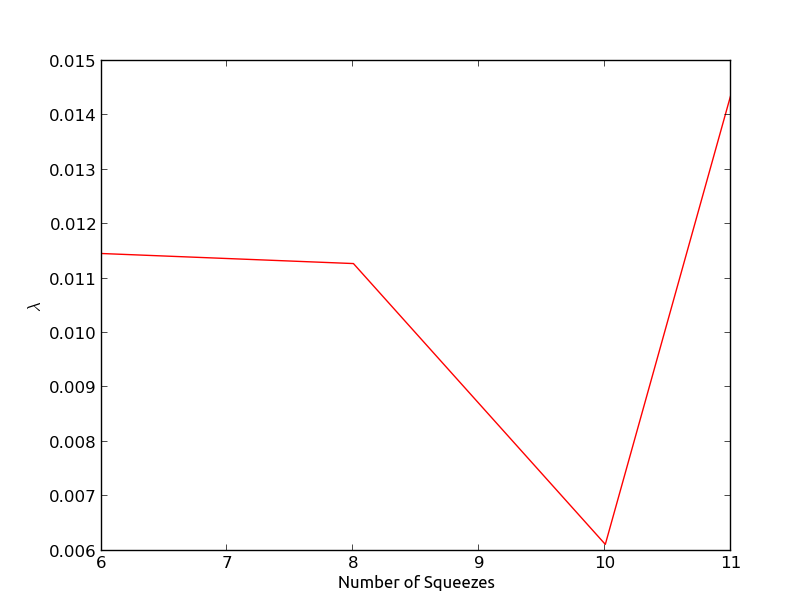
\includegraphics[width=2.5in]{plot3}
\caption{$\lambda$ versus number of squeezes at voltage 3000V.}
\label{fig:schematic}
\end{figure}

\begin{figure}[htbp]
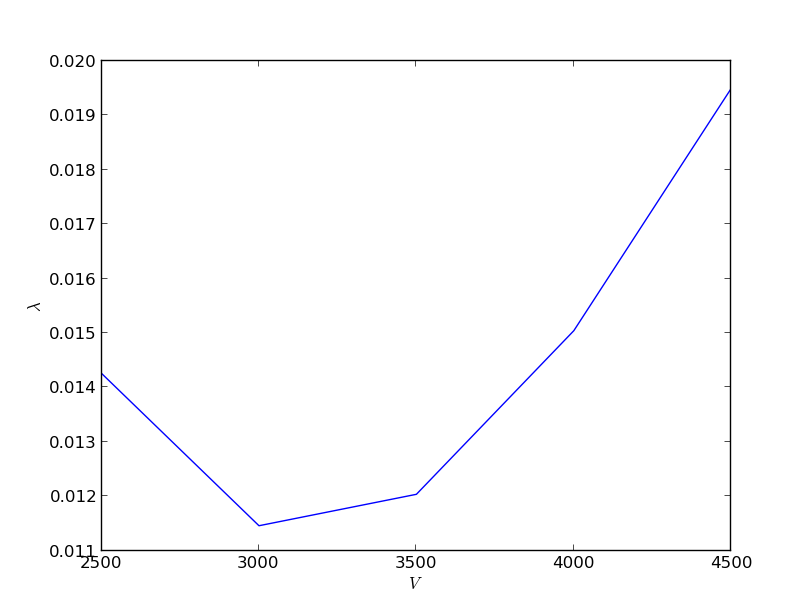
\includegraphics[width=2.5in]{plot4}
\caption{$\lambda$ versus $V$ in 6 squeezes.}
\label{fig:schematic}
\end{figure}

\section{Conclusions}
This experiment did not tell much things about radioactive decay since there would be a lot of causes of errors. For example, there were very few sample data to make good estimation and there were an irrelavence between them. My error shows this error explicitly. There is also no bound between numbers of squeezes, voltage value and $\lambda$.
This experiment showed us sometimes number of sample would be more helpful in making good estimations.


\section{References}

\begin{itemize}
\item E. Gulmez, ”Advanced Physics Experiment”, Istanbul, Bogazici University Publication, 1999
\item http://web.mit.edu/8.13/www/experiments.shtml
\end{itemize}

\bibliography{photoelectric}


%%%%%%%%%%%%%%%%%%%%%%%%%%%%%%%%%%%%%%%%%%%%%%%%%%%%%%%%%%%%%%%%%%%%%%%%%%%%%
\begin{acknowledgments} 

I would like to thank my partner Kadir Simsek for his help to the experiment, and also to the teaching assistant Merve Tarman for her guidance during the experiment.

\end{acknowledgments}

%%%%%%%%%%%%%%%%%%%%%%%%%%%%%%%%%%%%%%%%%%%%%%%%%%%%%%%%%%%%%%%%%%%%%%%%%%%%%

\end{document}
